\documentclass[german,a4paper,twoside]{scrreprt}
%\usepackage[ansinew]{inputenc}
\usepackage[utf8]{inputenc}
\usepackage[german]{babel}
\usepackage{makeidx}
\usepackage{graphicx}                      % Anleitung hierzu  in c:\Program Files\MiKTeX 2.7\doc\latex\graphics\grfguide.pdf
\usepackage{wrapfig}
%\usepackage[T1]{fontenc}
\usepackage{fancyhdr}
\usepackage[colorlinks]{hyperref}    % Bietet hyperlinks und Zugriffe auf Dateien in Farbe
\newcommand{\fspec}[1]{\protect\nolinkurl{#1}}
\makeindex
\parindent=0pt
\oddsidemargin=0.75\oddsidemargin
\evensidemargin=0.75\evensidemargin
%################# Ein paar Schreibvereinachungen ######################
\def\i{\itemsep=0.15\itemsep}
\def\c{\centering}
\def\bc{\begin{center}}
\def\ec{\end{center}}
\def\xc{\textsc{XCSoar~}}
\def\qo#1{\textsf{"#1"}}
\def\achtung{\marginpar{\includegraphics[height=3.0em]{Bilder/Achtung-Sign.jpg}}}
\def\merkes{\marginpar{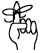
\includegraphics[height=3.0em]{Bilder/merkesdir.jpg}}}
\def\stop{\marginpar{\begin{center}
\includegraphics[height=2.50em]{Bilder/Stop.png}\\ {\footnotesize  \textbf{Stimmt das?}}\end{center}}}
\def\far{~{
\includegraphics[height=1.0em]{Bilder/farrowr.jpg}}~}
\def\fal{~{
\includegraphics[height=1.0em]{Bilder/farrowl.jpg}}~}
\def\blitz{ 
\includegraphics[width=1em]{Bilder/blitz1.png}}
\def\bblitz{\marginpar{
\includegraphics[height=2.0em]{Bilder/blitz1.png}}}
\def\bbblitz{
\includegraphics[height=4.0em]{Bilder/blitz1.png}}
\def\smallblitz{ 
\includegraphics[width=0.66em]{Bilder/blitz1.png}}
\rightmargin=0.55\rightmargin
\leftmargin=0.55\leftmargin

%----------------------------------------------------------------------------------------------
%----------------------------------------------------------------------------------------------
\begin{document}
\definecolor{buttongray}{rgb}{0.831,0.816,0.784}
\newcommand{\blink}[0]{$\triangleright$}
\newcommand{\bmenu}[1]{
	\fcolorbox {black}{buttongray}{{\sf{#1}}}
}
\newcommand{\bmenut}[2]{
	\fcolorbox {black}{buttongray}{
    \makebox[1.4cm][c]{
    	\begin{tabular}{c}
    	{\footnotesize\sf{#1}}\\
    	{\footnotesize\sf{#2}}
    	\end{tabular}
    }
  }
}
\newcommand{\bmenuth}[3]{
	\fcolorbox {black}{buttongray}{
    \makebox[1.4cm][c]{
    	\begin{tabular}{c}
    	{\footnotesize\sf{#1}}\\
    	{\footnotesize\sf{#2}}\\
    	{\footnotesize\sf{#3}}
    	\end{tabular}
    }
  }
}
\newcommand{\bmenus}[1]{
	\fcolorbox {black}{buttongray}{
    \makebox[1.4cm][c]{
      \begin{tabular}{c}
        {\footnotesize\sf{#1}}\\
    	  \\
      \end{tabular}
	  }
	}
}
\newcommand{\button}[1]{
	\fcolorbox {black}{buttongray}{{\sf #1}}
}

\newcommand{\infobox}[1]{
	\fcolorbox {black}{white}{\makebox[1.7cm][c]{\sf #1}}
}


\newenvironment{jspecs}{
\itemsep=2pt\topsep=3pt\partopsep=3pt\parskip=0pt
\begin{description}
\itemsep=2pt\topsep=3pt\partopsep=3pt\parskip=0pt
}
{\end{description}}

\newcommand{\jindent}[2]{
  \noindent\makebox[0pt][r]{{#1}\hspace*{\marginparsep}}
  \parbox[t]{0.95\linewidth}{#2}\par
}
                      %Lädt buttons, Menüs etc. von XCSoar - leicht variiert von OH.
\shorthandoff{"}                          %Anführungszeichen erscheinen wie auf Tastatur und nicht als Tastatursteuerzeichen.
\vspace*{2cm}

\begin{center}
  
\includegraphics[angle=0,width=0.5\textwidth,keepaspectratio='true']{graphics/logo.pdf}
  \vskip 0.5cm
  
\includegraphics[angle=0,width=0.66\textwidth,keepaspectratio='true']{graphics/title.pdf}
\end{center}

\vspace*{2cm}

\begin{center}
{\Large\textbf{\textsf{Flash\raisebox{-\baselineskip}[\ht\strutbox]{\bbblitz}Manual made by Hotte (OH)}}}\\
\end{center}
% \reflectbox{Spiegelverkehrt ?}? Ja, geht auch ... 
%\input{einleitung.tex}                                      % Fertig  bis auf die letzten 4 \sections
%\newpage
%\input{bedienerOF.tex}                                    % Noch gar nicht fertig ...
%\newpage
%\input{navigation.tex}                                     %fast fertig  für v6 machen
%\newpage
%\input{XC-Tasks.tex}                                       % Im Bau   für v6 machen ...
%\newpage
%\input{Endanflugrechner.tex}                         %Im Bau 
%\newpage
%\input{Athmosphaere-und-Instrumente.tex}   % Im Bau 
%\newpage
%\input{Airspace-und-Traffic.tex}                    % Im Bau 
%\newpage
%\input{Avionik-und-Airframe.tex}                    % Im Bau 
%\newpage
%\input{Schnellstart.tex}                                   %  Fertig.  % für v6 abändern-schon weit !
%\newpage
%\input{InfoBoxBeschreibung.tex}                    %  Im Bau Sehr Wichtig 
%\newpage
%\input{Konfiguration.tex}                               % Im Bau sehr wichtig   
%\newpage
\newpage
\section*{Vorwort}
"Von 0 auf \xc in weniger als 5 Minuten? Niemals." \\

Jeder, der mit der Version 5 oder früher noch gearbeitet hat wird dies sicher bestätigen können, denn die Konfiguration, ja allein die Auswahl der notwendigen Files für den Betrieb verschlang doch schon recht ordentlich Zeit.


 Inwzischen aber, dank der unglaublichen Arbeit des Entwicklungsteams hat sich derart viel getan, daß wir sagen können: "Na klar!"


 Folgt mir, und innerhalb von 5 Minuten, eine halbwegs schnelle Internetverbindung vorausgesetzt, \xc hilft Euch beim Fliegen. \\[2em]

Viel Spaß, OH
\chapter{Blitzeinstieg für die absolut Ungeduldigen}\index{Blitzeinstieg}\label{Blitzeinstieg}
\section{Voraussetzungen für den Betrieb}
Wir setzen hier einfach mal voraus, daß Ihr wißt, wie man mit einem \textsf{PDA}, \textsf{PNA}, \textsf{PC} oder aber dem  triadis \textsf{Altair} umgeht,  für den diese Software ursprünglich mal geschrieben wurde. Es soll hier nur die Software beschrieben werden, und zwar soweit, daß Ihr damit alleine Fliegen könnt.

Den Rest werdet ihr euch nach dieser kurzen Einweisung ganz sicher selber erarbeiten können, weil es wirklich kinderleicht ist.

Eine Bitte haben wir: es kann -und wird- immer wieder vorkommen, daß etwas falsch beschrieben ist, oder nicht so funktioniert, wie Ihr denkt, daß es soll, oder aber es ist tatsächlich ein handfester Fehler.\\[1em]

Werft das Programm bitte nicht gleich weg! \textsl{Gebt  uns eine Chance!}

Oder besser noch - \textsl{\textbf{macht mit!!!}} \xc ist ein Open Source-Programm. Das heißt, daß der Quellcode offen einsehbar und für und von jedermann nach Gutdünken veränderbar ist. Einzige Bedingung: Wenn Ihr es weitergebt, oder Teile davon benutzt, müßt Ihr den neuen Quellcode auch wieder frei verfügbar machen.\\

Wir tun dies aus der tiefen Überzeugung, daß Software nichts kosten muß um perfekt zu funktionieren.

Im Gegenteil. Dadurch, daß der Anspruch erst gar nicht aufkommt, Geld damit verdienen zu wollen, werden z.B.\ Dateiformate frei verfügbar und das auf der ganzen Welt.  Erinnert euch immer wieder an das elendige Update-Spektakel von einem auf das andere Datei-Format eines bekannten Textdokumentprogrammes, welches "alle zwei Jahre" ein neues Format - teilweise unlesbar für ältere Versionen - einführt, um Kunden in Abhängigkeit zu binden. Exakt so etwas wollen wir eigentlich nicht.\\

\xc ist  \textit{gratis}. Es kostet keinen Pfennig - im Gegensatz zu kommerziellen Programmen, welche sich derzeit im Bereich um die 150-200Taler bewegen. Es kann jeder (wirklich \textsl{jeder}) mitmachen, um es zu verbessern!

Also - wir freuen uns über jeden Beitrag und jede Rückmeldung, die uns hilft, das Programm besser zu machen - in Eurem und in unserem Sinne!\\[1em]


\large{\textbf{Und nun geht es los: }}\\[1em]

Um \xc  zum Laufen zu bringen, werden folgende Files benötigt:\index{Files, benötigte}\index{Wo finde ich die Files?}
\begin{enumerate}\i
\item das \xc -Programm, entweder als \texttt{CAB}-File (zur Installation) auf einem PDA, oder einfach als eigenständig laufendes \texttt{.exe} -File
\item Ein \texttt{xcm}-File. Hierin stehen Gelände (Berge, Seen) und Topologiedaten wie Straßen, Orte etc.\
\item Eine Luftraumdatei im \textsf{OpenAir}-Format. Eine solche stets aktuelle(!) bekommt ihr z.B.\ auf der Seite des \textsc{DAEC}, indem Ihr in z.B.\ eine bekannte Suchmaschine mit "\texttt{Luftraumdaten Deutschland download}" füttert.
\item Eine Wegpunkliste im Cambridge  \texttt{(*.dat)}, Zander  \texttt{(*.wpz)} und SeeYou \texttt{(*.cup)}-Dateien unterstützt.
Wegpunkte-Files sind z.B.\ erhältlich nach Eingabe in ebenjener Suchmaschine mit dem Stichwort "\texttt{welt2000}" oder aber direkt bei \url{http://www.segelfug.de/vereine/welt2000}
\end{enumerate}

Die Programm-Files findet ihr auf der Hompage von \xc \url{http://www.xcsoar.org}. Zum einen könnt Ihr das je nach Betriebssystem eigentliche Programm herunterladen, nach einem Klicken auf Download kommt Ihr auch zu den Karten, die Ihr Euch selber aussuchen könnt.
Auf den nächsten Abbildungen seht Ihr links die oben angegebene Hompage, rechts daneben - nachdem ihr auf Download geklickt habt, die Download Seite.
%
\begin{center}
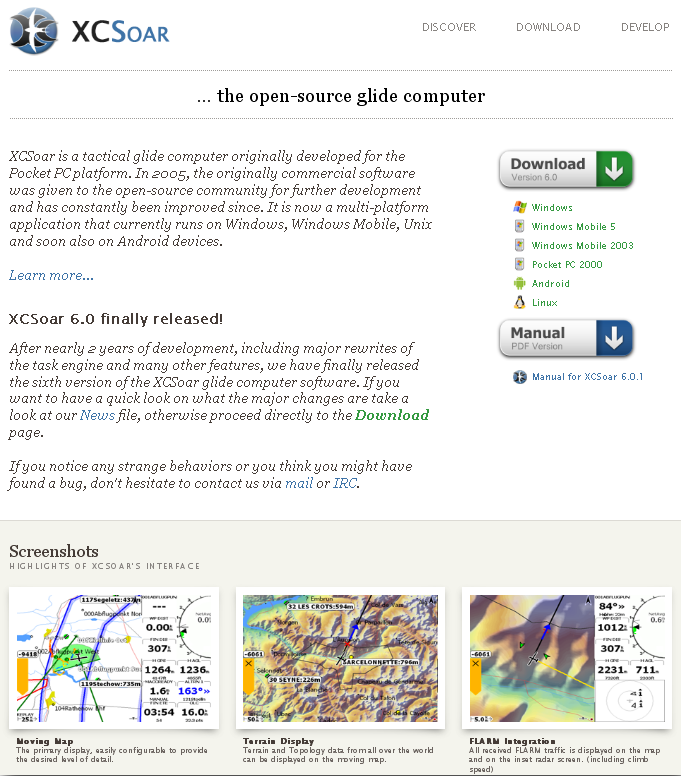
\includegraphics[width=7cm]{Bilder/XC-HP-HP.png}
\quad
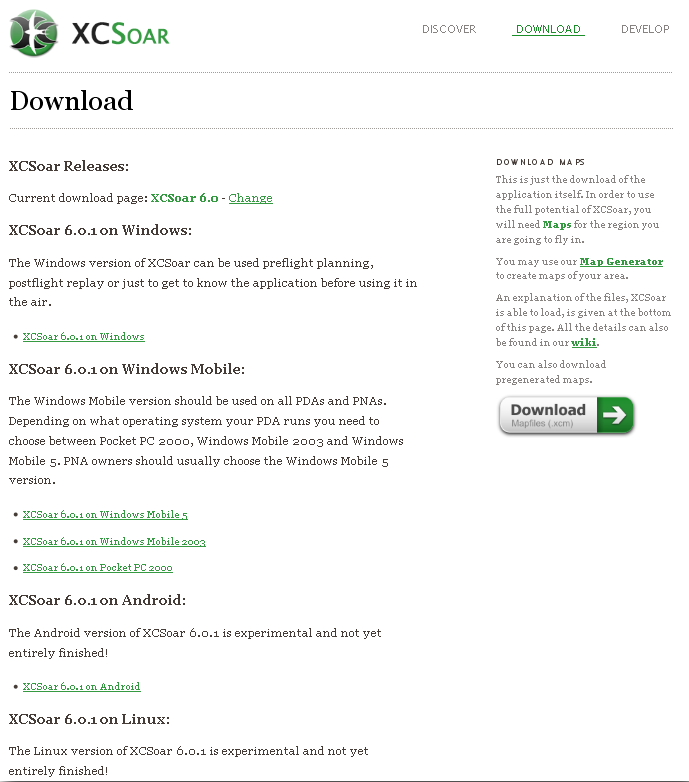
\includegraphics[width=7cm]{Bilder/XC-HP-Download.png}
\end{center}
%
Mit einem weiteren Klick auf Donwload gelangt Ihr auf die \textsf{Map}-Page, von der Ihr Euch letztlich die \texttt{xcm}-Files herunterladen könnt:
%
\begin{center}
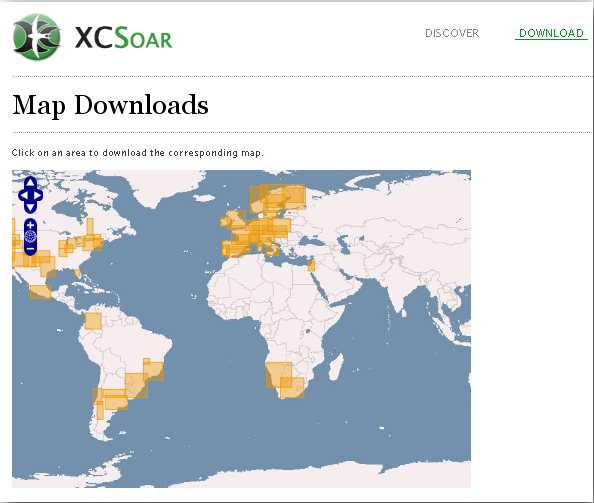
\includegraphics[width=11cm]{Bilder/XC-HP-MapDownload.png}
\end{center}
%

So. Wenn Ihr all die Files habt, kann es losgehen:\\[1em]

Speichert das \texttt{CAB}-File z.B.\ auf einer SD-Karte (tut Euch den Gefallen, und nehmt \textbf{schnelle} SD-Karten \footnote{(ohne Werbung machen zu wollen - ich nehme Sandisk Ultra, man merkt das wirklich deutlich - es gibt aber sicher auch schnelle Karten von Panasonic, Transend  und, und, und \dots - } wirklich!) und werft es \merkes auf Eurem \textsf{PDA} an. Das Programm wird  nun installiert und ein Ordner \texttt{XCSoarData} angelegt. \textbf{Alle} anderen oben genannten Files müssen anschließend in diesem Ordner stehen!

Alternativ könnt Ihr das \texttt{.exe} File irgendwo speichern und es separat anwerfen,
den Ordner \texttt{XCSoarData} manuell anwerfen. Sonst läuft nix.
%Der Ordner muß entweder in der root der SD-Karte liegen, oder  aber im MyDocuments-Ordner.
%
\section{Bedienung und Lesen dieser Anleitung}
Die Bedienung von \xc erfolgt entsprechend des Bedienkonzeptes der verwendeten Hardware.
Ein \textsf{PDA} z.B.\ kann mit den Hardwareknopf und der Wippe als auch dem Touchscreen
bedient werden. Ein \textsf{PNA} dagegen besitzt keine Knöpfe, sondern ist ausschließlich über den Touchscreen bedienbar.

Der \textsf{Altair} hingegen besitzt keinen Touchscreen und ist somit ausschließlich über Hardware buttons und Drehknöpfe bedienbar. Dennoch soll \xc auf allen Gerätetypen intuitiv, sicher und schnell bedienbar sein.

Diese Blitzanleitung ist daher so gestaltet, daß auf kürzest möglichem Wege die entsprechende Funktion gefunden werden kann. Die Konzentration liegt dabei auf der Bedienung des \textsf{PDA/PNA}.

Eine detaillierte Beschreibung werde ich evtl. noch nachreichen, wo wirklich alle Details beschrieben werden, jedoch ist das angesichts der rasanten Entwicklung von \xc wirklich schwierig\dots

Folgende Elemente will ich hier der Einfachheit verwenden:

\begin{tabbing}
\seite{Seitenansichten}\quad\=ökl\hfill \kill
\bmenut{Menü}{buttons} \> \parbox[c]{11,4cm}{Diese stellen die Hauptmenueinträge auf dem Touchscreen dar. In der Anleitung wird diese Darstellung benutzt, um einen Klick auf das
entsprechende Menu darzustellen. Zu Deutsch: Klickt drauf!}\\[1.2em]
\button{Buttons}           \>\parbox[c]{11,4cm}{Buttons sind Befehle innerhalb von Menüs.
Wenn so dargestellt wie  hier $\rightarrow$ draufklicken!}\\[1.2em]
\seite{Seitenansichten}  \>\parbox[c]{11,4cm}{Die gelb hinterlegten Texte sollen anzeigen, auf welcher Seite  Ihr Euch befindet. Das ist angelehnt bzw.\ exakt so, wie es auch in  \xc vorkommt. Kein Klick-nur Info!!}\\[1.2em]
\dklick                           \>\parbox[c]{11,4cm}{Ein Doppelklick irgendwo auf die Touchscreenoberfläche, jedoch \textsl{nicht} auf einen Wegpunkt.$\rightarrow$ Doppelklicken!}\\[1.2em]
\qquad\qquad \blink      \>\parbox[c]{11,4cm}{Naja, dies Zeichen soll heißen: als nächstes. Man hätte auch einen Pfeil oder sonstewas nehmen können\dots}
\end{tabbing}
%----------------------------------------------    ready   ----------------------------------------------------------
%-------------------------------------------------------------------------------------------------------------------
%-------------------------------------------------------------------------------------------------------------------
\subsection{Startbildschirm}\label{startbildschirm}
\begin{wrapfigure}{l}{4.4cm}
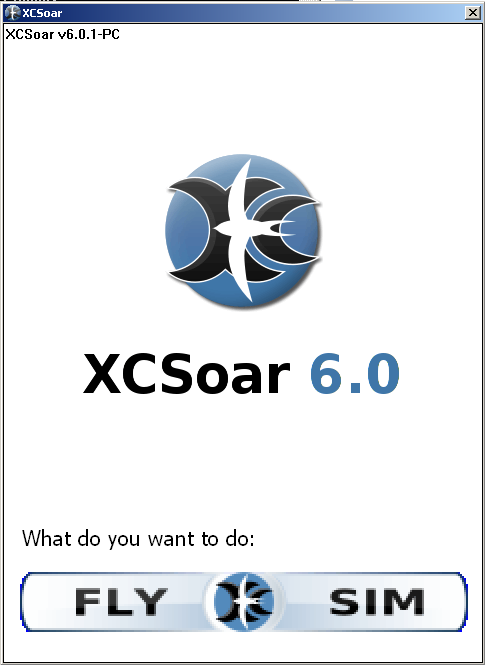
\includegraphics[width=4.5cm]{Bilder/ultrafirst.png}
\end{wrapfigure}
Das allererste, was Ihr seht, wenn ihr \xc gestartet habt ist der folgende Bildschirm:
Vollkommen klar, was damit gemeint ist. Es gibt eine Simulation \textsf{SIM}, mit der könnt Ihr herumspielen, um zu üben, und es gibt eine Version \textsf{Fly}, die ist für den "harten Überlandflugeinsatz".

Der einzige Unterschied ist der, daß in der Simulation keine GPS Daten empfangen werden müssen, so daß ihr z.B.\ Eure Flughöhe, und die Vorfluggeschwindigkeit, Wind und sowie McCready Wert etc.\ per Tasten einstellen könnt, um einen echten geplanten Flug zu simulieren und vor allem im Umgang sicher und schnell zu werden.


Siehe dazu unbedingt Kap.~\ref{sim-mode}, wenige Seiten weiter. Ich empfehle es \textbf{wirklich}, sich mit dem Simulationsmodus vertraut zu machen. Ist fast wie Flugsimulator, nur näher an der Realität, denn ihr seht hinterher genau dasselbe!

Nicht ist blöder, als im Flieger zu sitzen und grübeln zu müssen " \dots  mhhhhh -  das war doch\dots  irgendwie \dots ach sch\dots , dann flieg ich eben so weiter" Muß nicht sein. Echt nicht.  Der Winter ist ca. 5 Monate lang. da kann man sich - so nicht grade in Namibia oder Australien - mit dem \xc -Simulator (den gibt es nämlich auch für den PC! Natürlich auch gratis) top bekannt machen und fit in den Flieger steigen.

Sobald Ihr \xc dann startet (wir nehmen hier mal die \textsl{Sim}ulation), erscheint der folgende, weiße Bildschirm.


\begin{wrapfigure}{l}{4.4cm}
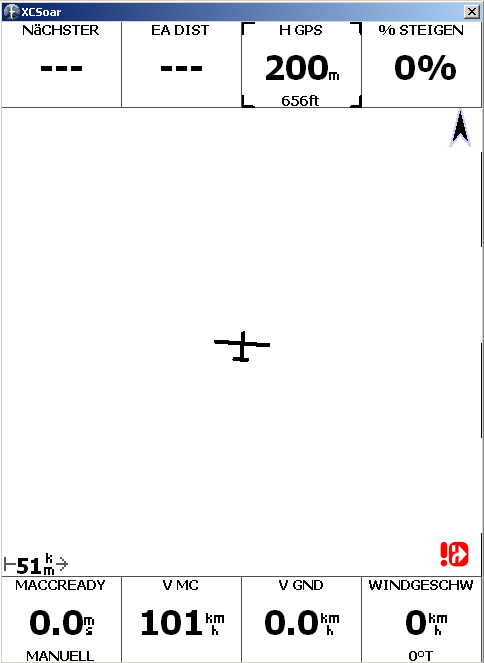
\includegraphics[width=4.5cm]{Bilder/veryfirst.png}
\end{wrapfigure}
Hiermit könnt Ihr im Prinzip noch nicht so fürchterlich viel anfangen, da Ihr ja eine \textsl{moving map} gewohnt seid und \textsl{zu recht} erwartet.

Die folgenden Schritte werde ich euch jetzt "pö a pö" bebildert durch dies Büchlein führen, auf daß ihr die Grundkonfiguration in weniger als 5 Minuten ohne "\textsl{HHHHmmmgrrrrmpff wie geht das jetzt ??}"  und " \textsl{ich schmeiß das Ding aus  dem Fenster raus !!}"  geschafft habt.

 Wie ihr dahin kommt, das genau wird jetzt ab hier schnell und ohne viel Erklärungen beschrieben  - ich hoffe, es fällt Euch nach dieser Beschreibung leicht, das Vorgehen nachzuvollziehen.\\

Ein \dklick bringt das folgende Bild zutage:
\begin{wrapfigure}{l}{4.4cm}
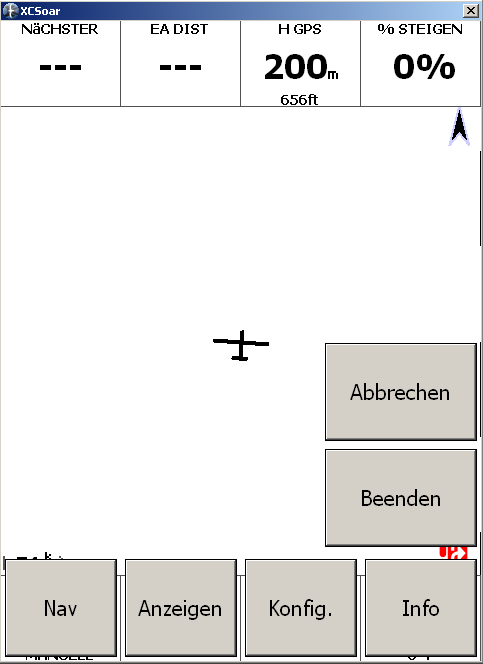
\includegraphics[width=4.5cm]{Bilder/verysecond.png}
\end{wrapfigure}
Hier seht Ihr unten vier graue Felder (Menüs, wie  oben beschrieben) und zwei größere rechts, deren Beschreibung ich  wohl nicht weiter beschreiben zu brauche. Das ist im Prinzip der Ausgangspunkt mit den vier Hauptmenüs, welche \xc bietet: \textsf{Nav}, \textsf{Anzeigen},\textsf{ Konfig.} und \textsf{Info}.

Zuallererst sollte man jetzt wissen, daß die vier Hauptmenüs \textsf{Nav}, \textsf{Anzeigen}, \textsf{Konfig.\ } und \textsf{Info} auf verschiedene Weisen aufgerufen werden können.\\

Es ist möglich, diese  \textsl{entweder }mit dem linken Hardwareknopf (\textsf{PDA}), per Doppelklick auf die Touchscreenoberfläche (\textsf{\textsf{PDA, PNA}}) oder einer der vertikal angeordneten, beschrifteten Druckknöpfe \textsf{Nav}, \textsf{Disp}, \textsf{Config} und \textsf{Info} (\textsf{Altair}) aufrufen.

Diese Hauptmenüs haben diverse Untermenüs, welche nacheinander auf dem Touchscreen
(\textsf{PNA,PDA}) oder dem Hardwareknopf (\textsf{PDA, Altair}) durchgklickt werden
können, bis der entsprechende Untermenüpunkt erreicht ist. Sind alle Menüpunkte
durchgeklickt, erscheint wieder der Bildschirm ohne Menüauswahl und man kann von
vorne loslegen.

Damit Ihr  \xc  überhaupt so einrichten und benutzen können wir ihr es wollt, müßt Ihr es \textsl{konfigurieren}. Und genau dazu gibt es das \textsf{Konfig.} - Menü.\\[1em]

Folgt mir -  versprochen:  \textsl{keine fünf Minuten!} -wenn ihr mir genau folgt bzw.\ bis hierher gefolgt seid!
%
\section{Übersicht Konfigurationsmenü-Menü}\label{Blitz-Konfig}\index{Blitzeinstieg, Konfiguration}
Da das Konfigurationsmenü für den Blitzeinstieg am wichtigsten ist, werden wir dies hier als erstes beschreiben. Das Menü hat eigentlich drei Hauptseiten, von dene ich hier aber nur zwei abbilde, denn die dritte Seite hat lediglich einen Eintrag(\textsf{Rohlogger}), welche für einen Blitzeinstieg jedoch unnötig ist und daher hier vernachlässigt wird:
\begin{center}
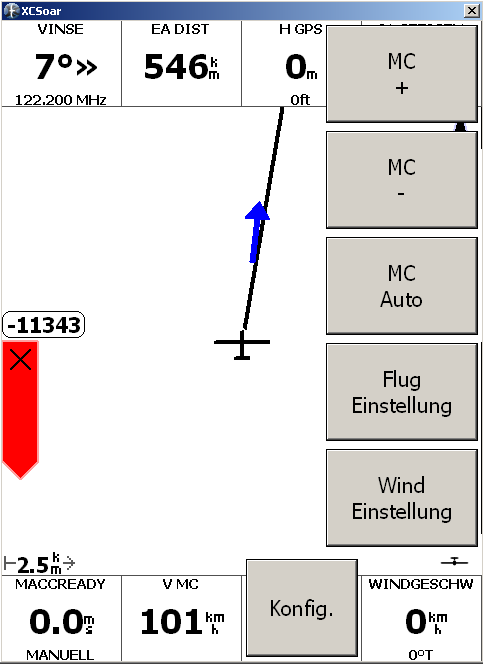
\includegraphics[width=4.5cm]{Bilder/HauptmenueKonfig1.png}%
\qquad\qquad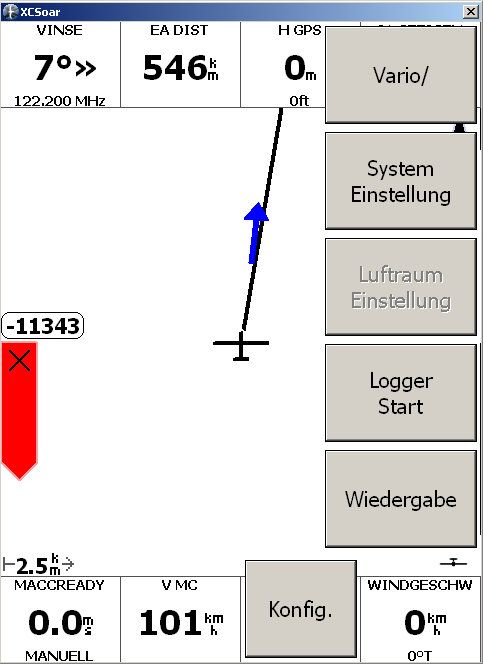
\includegraphics[width=4.5cm]{Bilder/HauptmenueKonfig2.png}
\end{center}

Das erste was Ihr jetzt macht, ist Eure Grundeinstellung, ähnlich des Vorflugchecks! Und das geschieht in den \textsf{Systemeinstellungen}!

Das Konfigurationsmenü \textsf{ Systemeinstellungen} erwartet Euch mit insgesamt 17 verschiedenen Seiten, die Ihr der Reihe nach mit \fal bzw.\ \far aufrufen und durchblättern könnt, um  \xc komplett an Eure Vorgaben/Vorlieben anpassen zu können. Ganz oben im Display erscheint immer gelb hinterlegt die Nummer der Seite und eine entsprechende Bezeichnung dazu. Für die Superkurzdarstellung der entsprechenden Befehle bzw. Tastenkombinationen setze ich jetzt immer einen \raisebox{0mm}[-0.20em][-0.5em]{\smallblitz} an den Rand.\\

\merkes\textit{Alle diese im Konfigurationsmenü eingestellten Werte erscheinen beim nächsten Start automatisch als vorgegebener Standard!}

 Ändern könnt ihr diese natürlich jederzeit. Es sei denn - und das ist wichtig zu wissen-, daß Ihr die \textit{Sicherheitssperre} \index{Sicherheitssperre} unter ~\ref{konfig11} unter "Sicherheitssperre"  eingeschaltet habt.
 Hierdurch ist es während des Fluges unmöglich, an der \xc -Konfiguration herumzufummeln.

 Dies dient Eurer Sicherheit !!! Einfach um Eure Aufmerksamkeit  während des Fluges nicht mit überflüssiger Fummelei  zu überlasten, welche Ihr sinnvollerweise vor dem Flug besser getan hättet.

 Ihr solltet während des Fluges \textit{rausschauen}, nicht am PDA kleben!!! Safety first, bitte!

Von jetzt ab möchte ich nicht mehr soo viel erzählen, sondern ihr könnt Euch anhand der folgenden Skizzen und  Kurzbeschreibungen weitestgehend ganz alleine durchklicken\dots

\subsection{Karten, Lufträume und Wegpunktdatein eingeben}\label{fileseingeben}\index{Map-Datei  eingeben}\index{Wegpunkt-Datei eingeben}\index{Luftraum-Datei eingeben}
\begin{center} \bblitz
\bmenus{Konfig}\blink~\bmenus{Konfig}\blink~\bmenut{System}{Einstellung}\blink~ \far \far \dots \qquad \seite{1 Platz}
\end{center}

Auf dieser Seite angelangt müßt bzw.\ könnt rechts neben \textsf{Landkarte} z.B.\ das File \texttt{Ger.xcm} angeben, damit habt Ihr schon mal die komplette Landschaft good old Germanys geladen. Den Rest tragt z.B.\ Ihr ein, wie nebenstehend oder so, wie \textsl{Eure Files eben heißen, die Ihr heruntergeladen} habt.


\begin{wrapfigure}{l}{4.4cm}
%\begin{wrapfigure}{r}{4.4cm}
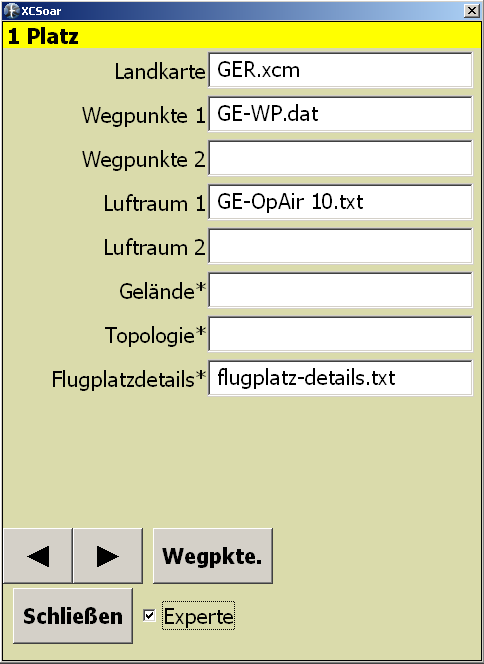
\includegraphics[width=4.5cm]{Bilder/Konfig1Platz.png}
\end{wrapfigure}
Nochmal mein Hinweis: Denkt daran, daß diese Files in \texttt{XCsoarData} stehen \textbf{und} das richtige Format haben!!! Sonst war es da mit den versprochen 5 Minuten!!\\

 Findet ihr beim Klicken auf das weiße Feld neben \textsf{Landkarte} kein File zur Auswahl, solltet Ihr sofort nocheinmal nachsehen, ob die Files das richtige Format haben (Nochmal zu Erinnerung - also Airspace: OpenAir-Format (ASCII-File), Wegpunkte: Cambridge-Format, SeeYou-Format oder Zander-Format der Ordner \texttt{XCsoar\-Data} existiert und ob die entsprechenden Files auch tatsächlich darin stehen. \\

 Wenn Ihr die Files entsprechend eingetragen habt, habt, dann klickt Ihr auf \button{Schließen}.
  Anschließend beendet und startet Ihr \xc neu. Mehr braucht Ihr eigentlich nicht. (Das Kreuzchen neben Experte muß Euch hier nicht stören, das ist für zusätzliche Files gedacht und Ihr könnt es für den Blitzeinstieg auch wegklicken\dots )

Euer \xc sollte bereits jetzt soweit konfiguriert sein, daß Lufträume, Gelände, Flüsse und Wegpunkte bekannt und auch sichtbar sind.\\

Nun interessiert Euch mit Sicherheit als allererstes, wie Ihr Euren Heimatflugplatz als Start- und Landeplatz oder als Standardplatz aktivieren könnt. Dazu ein paar Seiten weiter siehe Kap.\ \ref{Heimatflugplatz}. Naklar - wenn das erledigt ist, seit Ihr sicher ungeduldig und wollt den ersten Task eingeben.
Mehr dazu siehe Kap.\ \ref{Irgendeinzieleingeben} oder \ref{aufgabeeingeben}.

Wir machen hier kurz noch weiter mit der Eingabe der Polare und so unwichtigen Dingen wie Sprache, Namen, Kennzeichen etc.\  eingeben

\subsection{Sprache einstellen}\index{Sprache einstellen}\label{Spracheeingeben}
\begin{center}
 \bmenus{Konf.}\blink~\bmenus{Konf.}\blink~\bmenut{System}{Einstellung}\blink~\far \far\dots\seite{11 Benutzeroberfläche}
 \end{center}

 \textsf{Sprache}: Sprache wählen. Bei \textsf{Voreinstellung} wählt  \xc die  Sprache Eures Betriebssystemes.
 \stop

\subsection{Polare eingeben}\index{Polare eingeben}
\begin{center}
\bmenus{Konfig}\blink~\bmenus{Konfig}\blink~\bmenut{System}{Einstellung}\blink~ \far \far \dots \qquad \seite{8 Polare}
\end{center}
Hier angelangt wählt Ihr im Feld \textsf{Polare} Euren Flieger aus. Oder aber Ihr wählt den
Eintrag \textsf{External Polar File}. Damit könnt Ihr eine eigene Polare eingeben, falls Eure nicht vorhanden ist, oder nicht paßt. Diese Datei \textbf{muß} im \textsf{WinPilot}-Format vorliegen.
Eine entsprechende Vorlage könnt Ihr Euch bei einer beliebigen, hier nicht näher genannten Suchmaschine aus dem Netz saugen.

\subsection{Flugzeugtyp und Name}\index{Flugzeugtyp eingeben}\index{Pilotenname eingeben}\index{Wettbewerbskennzeichen eingeben}
\begin{center}
\bmenus{Konfig}\blink~\bmenus{Konfig}\blink~\bmenut{System}{Einstellung}\blink~ \far \far \dots \qquad \seite{16 Logger}\bblitz
\end{center}
In diesem Menü angelangt, könnt Ihr Euren Namen, den Flugzeugtyp und die Kennung angeben.


%----------------------------------------------    ready   ----------------------------------------------------------
%-------------------------------------------------------------------------------------------------------------------
%-------------------------------------------------------------------------------------------------------------------
\section{Übersicht Anzeige-Menü}\label{Blitz-Anzeige}
to be written\dots
%----------------------------------------------    ready   ----------------------------------------------------------
%------------------------------    to be continued  ---------------------------------------------------------------
%-------------------------------------------------------------------------------------------------------------------
\section{Übersicht Info-Menü}\label{Blitz-Anzeige}
to be written\dots
%----------------------------------------------    ready   ----------------------------------------------------------
%-------------------------------------------------------------------------------------------------------------------
%-------------------------------------------------------------------------------------------------------------------
\section{Übersicht Nav-Menü}\label{Blitz-Nav}
Das \textsf{Nav}-Menü  hat zwei Seiten. Man kann es, wie alle anderen Menüs auch, entweder mit dem linken Hardwareknopf (\textsf{PDA}), per Doppelklick auf die Touchscreenoberfläche  (\textsf{\textsf{PDA, PNA}}) oder mit dem oberen linken Druckknopf: \textsf{Nav} (\textsf{Altair}) aufrufen.

Das linke Bild zeigt die erste Seite des \textsf{Nav}-Menüs, rechts ist die zweite Seite gezeigt. Eine dritte gibt es bisher noch nicht, was natürlich nicht heißt, daß es sie nicht irgendwann mal geben wird. .
\begin{center}
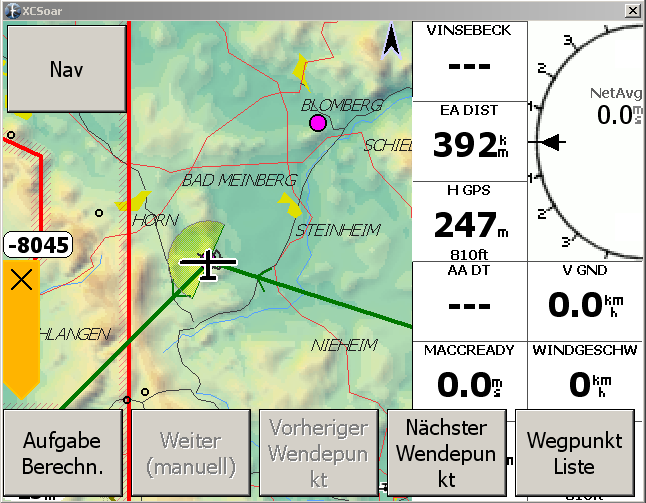
\includegraphics[width=5.5cm]{Bilder/Nav-Menu1.png}
\qquad
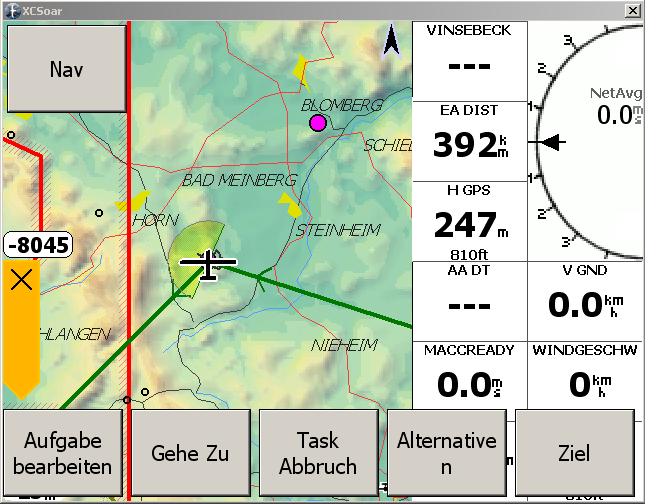
\includegraphics[width=5.5cm]{Bilder/Nav-Menu2.png}
\end{center}

%----------------------------------------------    ready   ----------------------------------------------------------
%-------------------------------------------------------------------------------------------------------------------
%-------------------------------------------------------------------------------------------------------------------
\subsection{Heimatflugplatz eingeben}\index{Heimatflugplatz eingeben}\label{Heimatflugplatz}
\begin{itemize}
\item \bmenus{Nav} \blink~\bmenut{Wegpunkt}{liste}\blink~\seite{Wegpunktauswahl}\blink~ \button{Name}
\item \textsf{VIN} mit der eingeblendeten Tastatur eintippen  \blink~ \button{Ok}
\item \textsf{Vinsebeck}~\dklick bzw.\ \button{Auswählen} \blink~\seite{Wegpunktinfo 'Vinsebeck Fran'}\far
\item \button{Setze als neuer Heimatplatz}
\end{itemize}
\begin{center}
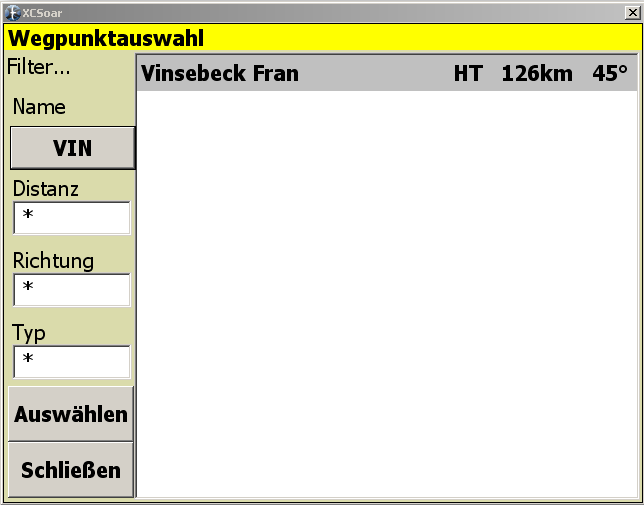
\includegraphics[width=5.5cm]{Bilder/Wegpunkt-Auswahl2.png}\qquad%
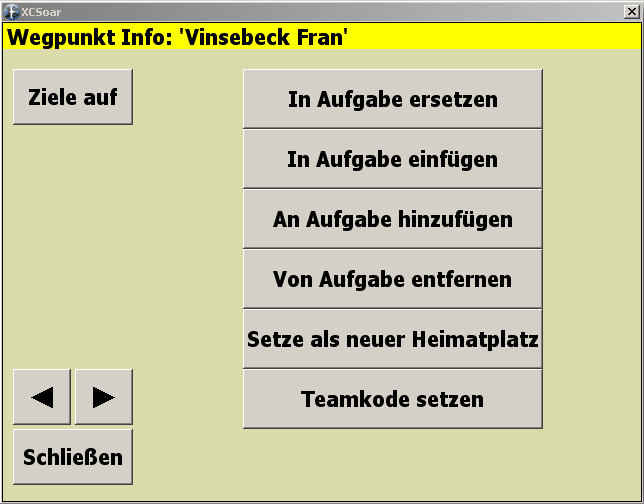
\includegraphics[width=5.5cm]{Bilder/Wegpunkt-Info2.png}
\end{center}
Alternativ ist das folgende Vorgehen ebenfalls möglich,
\begin{itemize}
\item \dklick des gewünschten  \textsf{Wegpunktes} auf der Touchscreenoberfläche. Es öffnet sich das Fenster \seite{Wegpunkt Info} mit dem entsprechend ausgewählten Wegpunkt.
\item \far  unten am Bildschirmrand  anklicken
\item  \button{Setze als neuer Heimatplatz}
\end{itemize}
%------------------------------------  ready     -------------------------------------------------------------------
%-------------------------------------------------------------------------------------------------------------------
%-------------------------------------------------------------------------------------------------------------------
\subsection{Irgendein Ziel angeben}\index{Ziel eingeben}\label{Irgendeinzieleingeben}
Zwei grundsätzliche Möglichkeiten:

\begin{itemize}
\item \bmenus{Nav}\blink~\bmenut{Wegpunkt}{liste}\blink~\seite{Wegpunktauswahl}
\item Wegpunkt über die vier Filter\ref{wegpunktfilter} (Name, Typ, Distanz, Richtung) auswählen mit Doppelklick oder \button{Auswählen} \blink~\button{Ziele auf}
\end{itemize}

oder

\begin{itemize}
\item \dklick auf einen Wegpunkt auf der Touchscreenoberfläche. Es öffnet sich das Fenster \seite{Wegpunkt Info} mit dem entsprechend ausgewählten Wegpunkt.
\item Unten am Bildschirmrand auf \button{Ziele auf} drücken.
\end{itemize}


%----------------------------------------------    ready   ----------------------------------------------------------
%-------------------------------------------------------------------------------------------------------------------
%-------------------------------------------------------------------------------------------------------------------
\subsection{Eine Aufgabe eingeben}\label{aufgabeeingeben}
\begin{center}
\bmenus{Nav}\blink~\bmenus{Nav}\blink~\bmenut{Aufgabe}{bearbeiten}
\end{center}
\begin{itemize}
\item \button{Bearbeiten}
\item \button{Neu}
\item Aufgabentyp wählen. (Ich wähle hier mal \textsf{FAI Dreieck})
\item \button{Wegpunkt hinzufügen} Wegpunkt über die vier Filter\ref{wegpunktfilter} (Name, Typ, Distanz, Richtung) auswählen.
\item Typ des Wegpunktes festlegen. (Ich wähle \textsf{Abfluglinie})
\item Wegpunktauswahl  mit \button{OK}  und \button{Auswahl} bestätigen.
\item nächste(n) Wegpunkt(e) hinzufügen (siehe oben), hierbei Typ (Sektor oder Zylinder) angeben
\item Zielpunkt angeben
\item Aufgabe speichern (! nicht vergessen!)
\end{itemize}

%----------------------------------------------    ready   ----------------------------------------------------------
%-------------------------------------------------------------------------------------------------------------------
%-------------------------------------------------------------------------------------------------------------------
\subsection{Task unterbrechen und zurück zum Task (Ausweichflugplatz)}\index{Task unterbrechen}\index{Task zurückkehren}\index{Task fortsetzen}
Task abbrechen und anderen Ausweichplatz/Landestelle suchen:
Sämtliche Berechnungen  erfolgen nun bezüglich des gewählten Wegpunktes.

Entweder:
\begin{center}
\bmenus{NAV}\blink~\bmenus{NAV}\blink~\bmenut{Task}{Abbruch} \bblitz
\end{center}
Der aktive Task wird ausgeblendet und es erscheinen \textsl{alle erreichbaren Plätze} magenta markiert mit grünem Ring, von denen man sich einen wie oben beschrieben auswählen kann.

Man kann aber auch \textsl{direkt} einen Platz anwählen, welcher evtl. \textsl{noch nicht erreichbar} ist:
\begin{center}
\bmenus{NAV}\blink~\bmenus{NAV}\blink~\bmenus{Gehezu} \bblitz
\end{center}
Anschließend Wegpunkt über die vier Filter\ref{Filter} (Name, Typ, Distanz, Richtung) auswählen mit Doppelklick oder \button{Auswählen} \blink~\button{Ziele auf}

Wenn der Task anschließend wieder fortgesetzt werden soll:
\begin{center}
\bmenus{NAV} \blink~\bmenus{NAV} \blink~\bmenut{Task}{fortsetzen} \bblitz
\end{center}
Sämtliche Berechnungen erfolgen wieder gemäß des vorher gewählten Tasks.
Dies Spielchen kann beliebig oft wiederholt werden, bis man sich anhand von
Ausweichflugplätzen zurück nach  Hause gemogelt hat\dots
%----------------------------------------------------------------------------------------------------------------
%----------------------------------------------------------------------------------------------------------------
%----------------------------------------------------------------------------------------------------------------
\subsection{AAT - Wegpunkt verschieben}
\begin{center}
\bmenus{NAV}\blink~\bmenus{NAV}\blink~\bmenus{Target}\blink~\seite{Ziel}\bblitz
\end{center}
In laufender Aufgabe folgende benutzt Ihr Tasten/Schaltflächenkombination. Ihr befindet Euch dann hier auf der \textsf{Ziel}-Seite mit allen Wegpunkten der aktuellen Aufgabe - siehe die nächsten Bilder. Auf dem linken Bild seht Ihr, daß \textsf{Auto} angeklickt ist, dementsprechend rechnet \xc für Euch den optimalen Weg - wenn es das Wetter und die Wolken denn zulassen. Auf dem rechten Bild ist  \textsf{Locked} angeklickt und nur so kann der  Punkt manuell verschoben werden. Automatisch haben sich Ankunftszeit, Zeitdifferenz etc. mit geändert\dots.
\begin{center}
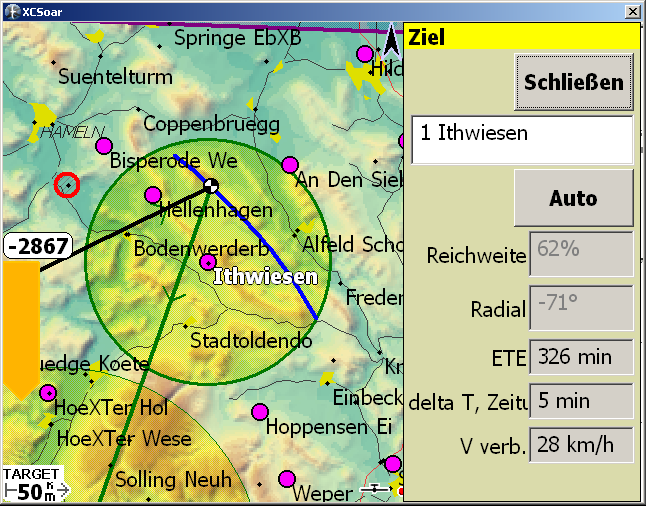
\includegraphics[width=5cm]{Bilder/AAT-Verschieb0.png}%
\qquad
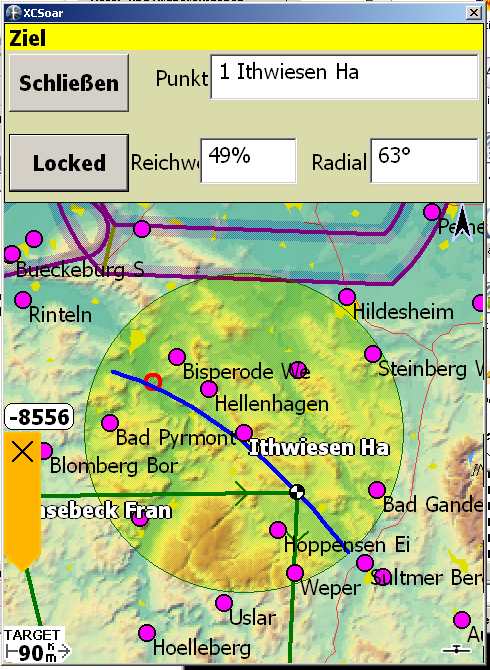
\includegraphics[width=5cm]{Bilder/AAT-Verschieb1.png}%
\end{center}
Denkt dran, den Punkt bei Bedarf nachzuverschieben, damit Ihr nicht zu früh ankommt, nachdem Ihr die Automatik abgestellt habt! Ebenso möglich ist es, \textsl{entweder} das Radial und/oder die Entfernung in den weißen Fenstern zu ändern. Ich wüßte aber nicht, wann ich das je tun sollten, denn ich schaue lieber raus und verschiebe die Punkte nach dem Wetter - nicht nach Winkeln, oder Entfernungen.
Das ist meiner Meinung nach meist besser, denn\xc kann beim besten Willen nicht die Wolkenentwicklung vorhersehen und beurteilen, wo die Wende -abhängig vom Wetter- am sinnvollsten wäre. Aber wer weiß, evtl. gibt es ja auch Piloten, die das gerne und erfolgreich benutzen\dots
%
\subsection{Texteingabe und Auswahlfilter (Wegpunkt-Typfilter)}\index{Texteingabe}\index{Wegpunkt-Typ-Filter}\label{Texteingabe}\label{Filter}
\begin{center}
\bmenus{Konfig.}\blink~\bmenus{Konfig.}\blink~\bmenut{System}{Einstellungen}\blink~\seite{11 Benutzeroberfläche}\blink~\button{Texteingabestil}\\[1em]
 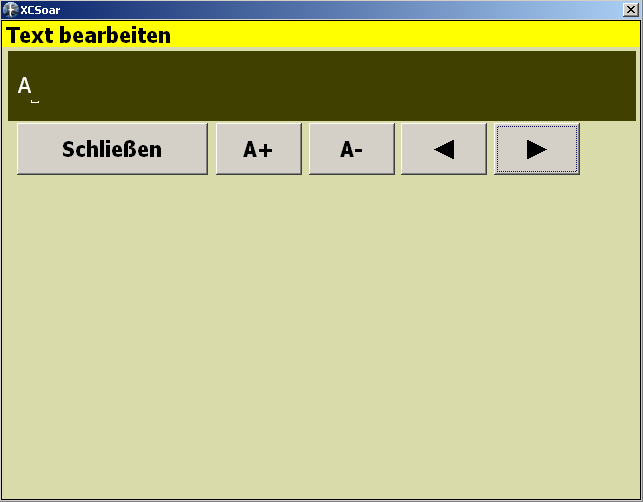
\includegraphics[width=6cm]{Bilder/Texteingabe2.png}\qquad 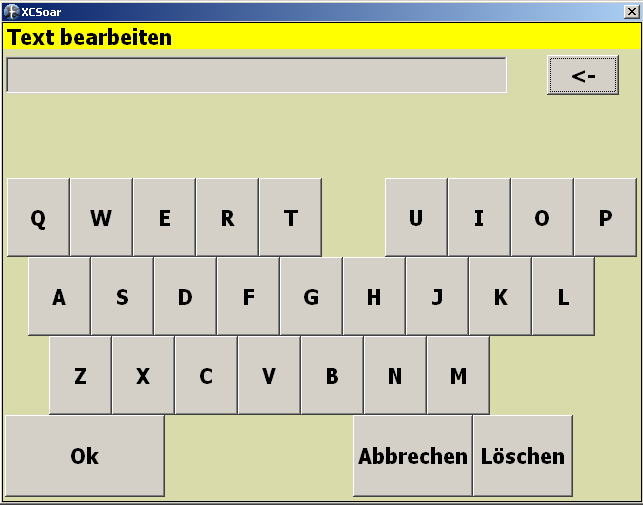
\includegraphics[width=6cm]{Bilder/Texteingabe1.png}
\end{center}
Ihr könnt in \xc sehr komfortabel Text eingeben.  Als Standard ist folgendes Verfahren vorgegeben, welches Ihr jedoch (wer hätte das gedacht\dots) in der Systemkonfiguration unter Benutzeroberfläche, Kap.\  \ref{Konfig11} ändern könnt. Wir möchten zum Beispiel in \textsf{Vinsebeck} starten und drücken dementsprechend im Text bearbeiten-Fenster auf \button{Name}.

\xc bietet hier eine sogenannte\textsl{ inkrementelle Suche}, was bedeutet, daß zuerst alle Flugplätze mit
dem ersten Buchstaben gelistet werden, anschließend der zweite, dann der dritte, so daß spätestens nach
dem dritten oder vierten Buchstaben der gewünschte Platz zur Auswahl bereit steht.

Wir drücken hier der Reihe nach \textsf{V, I, N} und sehen, wie oben im grauen Feld  (unter \textsf{Text bearbeiten})
die Buchstaben \textsf{VIN} erscheinen.  Alternativ steht (links im Bild) die
sog.\ Ranglisteneingabe zur Verfügung, welche per Cursorbewegungen einzeln die Buchstaben hochzählt.
Wer's lieber mag\dots

Die Filterfunktion für Wegpunkte von \xc macht es Euch extrem leicht, auch im Fluge Wegpunkte schnell zu finden.
Es stehen vier Filter \textsf{Typ}, \textsf{Name}, \textsf{Distanz} und \textsf{Richtung} zur Verfügung, die Ihr auswählen bzw. einschränken könnt.

Ein Klick auf \textsf{Typ} und Ihr könnt die Wegpunktauswahl einschränken in diverse Kategorien, welche wohl ziemlich selbsterklärend sind. Im Beispiel unten seht Ihr die Wegpunktseite und anschließend den Filter \textsf{Distanz}aufgerufen:

\begin{center}
\bmenus{Nav}\blink~\bmenut{Wegpunkt}{Liste}\\

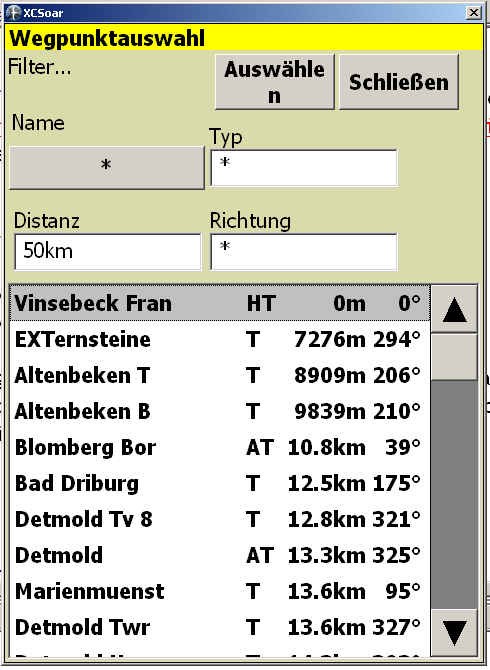
\includegraphics[width=5.5cm]{Bilder/WegpunktauswahlDistanz.png}\qquad
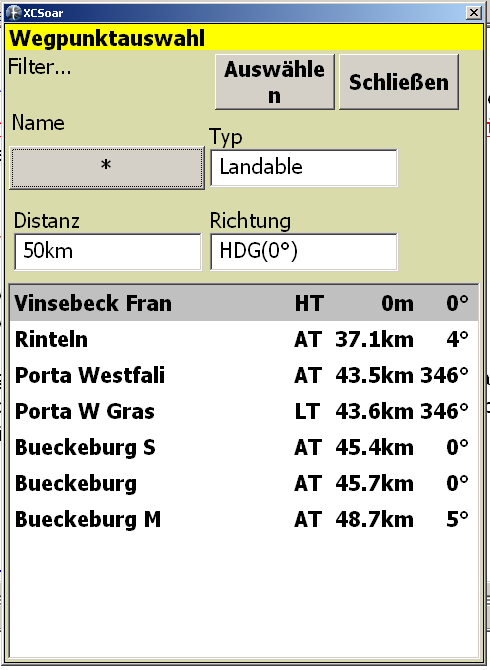
\includegraphics[width=5.5cm]{Bilder/WegpunktauswahlTypRichtungDistanz.png}
\end{center}

Die linke Auswahl per \textsf{Distanz} ermöglicht es Euch, alle Wegpunkte zu wählen, die innerhalb einer gewissen Entfernung um Euch herum liegen. Es sind auch Kombinationen möglich, also z.B.\ die Wahl von \textsf{Typ}, \textsf{Distanz} und \textsf{Richtung}. Das braucht, denke ich keiner weiteren großen Erklärung.

Die Reihenfolge der Anzeige ist denkbar einfach:
\begin{itemize}\i
\item Wenn die \textsl{Distanz} als Auswahlkriterium mit angegeben ist, dann werden immer alle Wegpunkte nach der Entfernung geordnet beginnend angezeigt, also der nächstliegende zuerst.
\item Ist nur \textsf{Name} angewählt, so werden die Plätze alphabetisch angeordnet.
\item Die Auswahl von \textsl{HDG} (Heading, also Vorauskurs) im Feld \textsl{Richtung} zeigt Euch alle Wegpunkte an, die in einem Winkel von ca. $\pm$ ca.\ $15^\circ$ zu Eurer aktuellen Flugrichtung, der Entfernung nach geordnet, liegen.
\end{itemize}

\section{Simulationsmodus}\label{sim-mode}\index{Simulationsmodus}
Der Simulationsmodus ist eine riesengroße Hilfe, um sich mit \xc vertraut zu machen!

Alle Anzeigen, Manöver, Tasks, Lufträume und das komplette Verhalten und Bedienung von \xc werden exakt
so dargestellt, wie später auch in der \textsl{FLY}-Version. Das einzige, was eben nicht geht, ist die exakte Bestimmung der Position mittels GPS und damit auch alle anderen "Echtzeitdaten", wie z.B. Geschwindigkeit und Höhe.

Aber auch dafür gibt es Abhilfe:
\subsection{Simulator: Starten und Landen, Höhe, MC-Wert eingeben etc\dots }\label{SimStartenLanden}
Um einen Flug im Simulator zu \textit{starten} zu können, geht Ihr wie folgt vor:
\begin{itemize}
\item Starten von \xc im \textsl{SIM}-Modus gemäß~\ref{startbildschirm}
\item Auf die gewünschte Infobox  am oberen bzw.\ unteren Rande des Bildschirmes z.B.\ (\textsf{MC}, \textsf{V Gnd},\textsf{H  GPS} und einige andere sind edierbar, aber nicht alle!) klicken.
\item Anschließend diese Werte mit der Wippe (hoch und runter) verändern.
\end{itemize}
Zur Bestätigung, daß Ihr im "Einstellungsmodus" zum Verändern der Werte seid, erscheinen um die Infobox vier kleine Ecken.

Um weiterzumachen $\rightarrow$ \dklick und Ihr könnt die Richtung des Flugzeuges mittels drücken und ziehen mit des Stiftes oder Fingers auf der Oberfläche in die entsprechende Richtung verändern.

Klickt auf die \infobox{V Gnd}-Box und ab ca. 90km/h erfolgt die Meldung : "Abgehoben" $\Longrightarrow$ Ihr fliegt! Bringt Ihr die Geschwindigkeit wieder unter ca.\ 90km/h, so erfolgt nach einigen Sekunden die Meldung "Gelandet" auf dem Bildschirm.
\begin{center}
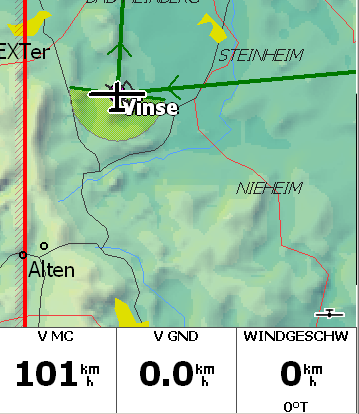
\includegraphics[width=4.5cm]{Bilder/SimInfoBoxNaktiv.png}%
\qquad
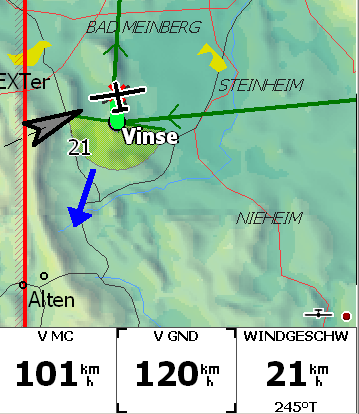
\includegraphics[width=4.5cm]{Bilder/SimInfoBoxAktiv.png}%
\end{center}
Links seht Ihr die nicht angewählte Infobox \infobox{V GND},rechts die angewählte Box, frei zum Verändern, markiert durch die Ecken.  Zusätzlich hab ich mal ein bißchen Wind spendiert (s.~\ref{SimuWind}, auf daß die Egge trägt (leider an der falschen Seite)  :-(

Jetzt könnt Ihr noch die Höhe einstellen \infobox{H  GPS}, und, falls Ihr vorher die Darstellung Eures Gleitbereichs eingestellt habt, könnt Ihr erkennen,
wie weit ihr mit dieser Höhe \textit{circa} kommen würdet (je nach Einstellung im Konfigurationsmenü 6 unter
%Kap.~\ref{Konfig6}
"Gleitflugbereich als" $\rightarrow$ Linie, schraffierter Bereich oder nichts). Die Linie oder der Bereich schrumpft oder wächst augenblicklich mit\dots

Stellt Ihr nun noch den MC-Wert ein, so werdet ihr merken, wie sich eure Ankunftshöhe und/oder -zeit hierzu entsprechend ändert. Kurzum, Ihr könnt hier phantastisch mit herumspielen und Euch in der Bedienung üben, solange das Wetter mies ist. Fit im Umgang mit den Instrumenten bedeutet weniger Belastung und Streß im Flug. \xc soll eine Hilfe sein, kein Selbstzweck!

Erstellt einfach einen Task, speichert ihn ab, ladet ihn und fliegt mal eine Runde.
\subsection{Simulator: Wind einstellen}\label{SimuWind}\index{Wind einstellen}
\begin{center}\bblitz
\bmenus{Konfig.}\blink~\bmenut{Wind}{Einstellung}\blink~\raisebox{-1.5cm}[]{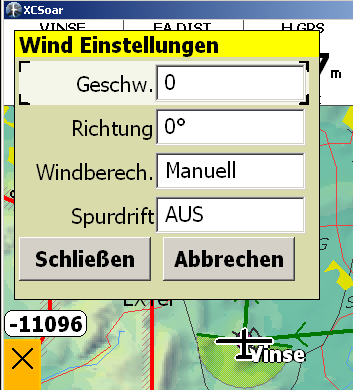
\includegraphics[width=3.5cm]{Bilder/WindEinstellungen.png}}\\[0.3em]
\end{center}
Normalerweise errechnet \xc aus dem Kurbelversatz oder aber durch den Versatz  im ZickZack-Flug die Windrichtung und -geschwindigkeit.  Im Rechner am Boden im Wohnzimmer gibt es leider keinen Versatz und auch keine Windgeschwindigkeit, von offenen Türen abgesehen. Dennoch - auch im Simulationsmodus könnt Ihr mit dem Wind fliegen! Die Einstellung hierfür erfolgt exakt genauso, als ob Ihr im Flugzeug sitzt, und den Wind manuell eingeben wollt, siehe obiger Auschnitt aus dem Display.
\begin{center}  \textbf{Wichtig!!}  \end{center}
Im Feld \textsl{Windberechnung} müßt Ihr hier, \textsl{im Simulator unbedingt \textbf{manuell}} anklicken, ansonsten tut sich nichts und \xc wartet vergebens auf irgendeinen Kurbelversatz.

Habt Ihr nun den Wind mit Richtung und Geschwindigkeit angegeben, so werdet Ihr bei genauer Betrachtung feststellen, daß sich etwas an der Bildschirmdarstellung geändert hat siehe auch zum Vergleich die beiden Bilder in Kap.~\ref{SimStartenLanden}.
 \begin{enumerate}
  \item Es erscheint ein hellgrauer Pfeil mit der Spitze zeigend auf Euer Flugzeug, der Euch die Windrichtung angibt
  \item Nahe am Pfeil wird die Windgeschwindigkeit angegeben, und zwar in der Einheit, welche Ihr im Konfigurationsmenü 10 eingestellt habt.
%      unter  Kap.~\ref{Konfig10} eingestellt habt.
  \item Die Darstellung des Geländes hat sich verändert!
  Die Luvseite von Bergen und Hügeln erscheint hell, die Leeseite dagegen dunkel geschummert.
  Natürlich können nicht alle lokalen Windverhältnisse wie Brise, Mistral oder gar Welle, wie sie z.B.\ massiv
  in Südfrankreich auftreten dargestellt werden, immerhin jedoch ist das ein netter Anhaltspunkt für eine
  schnelle grobe Beurteilung der Windverhältnisse.

  Im \textsf{Fly}-Modus wird durch die Kalkulation des Windes während des Fluges diese Richtung permanent
  aktualisiert. Natürlich ist auch diese Funktion im Konfigurationsmenü 6 unter
  %~\ref{Konfig6}
  "Windberech." konfigurierbar.
 \end{enumerate}
 Sehr deutliche Windveränderungen in Richtung und/oder Geschwindigkeit , z.B.\ durch Windscherungen, werden durch eine  Meldung "Erhebliche Windänderung" nach einigen Sekunden auf dem Bildschirm  angezeigt.
%%\begin{minipage}[position]{width}
%text
%\end{minipage}
\subsection{Konfigurationsmenü 1 - Platz}\label{Konfig1}
\begin{wrapfigure}{l}{4.5cm}
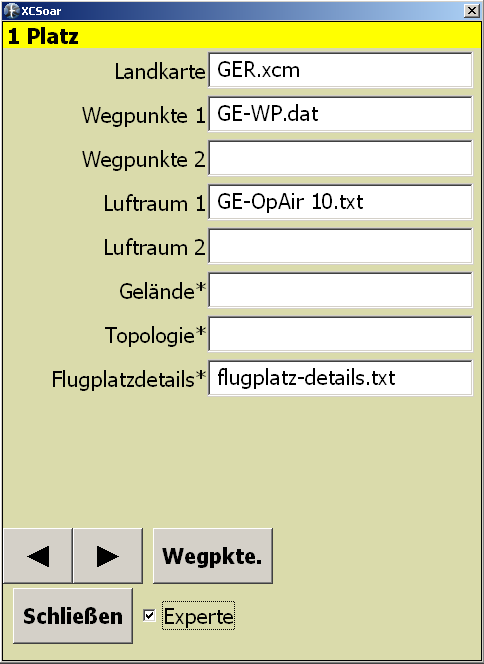
\includegraphics[width=4.5cm]{Bilder/Konfig1Platz.png}
\end{wrapfigure}
\textsf{Landkarte} Auswahl der Landkarte, welche benutzt werden soll. (\texttt{.xcm})-Format. Hierin enthalten ist bereits die Topologie mit Seen, Flüssen und Städten\\[0.5em]
\textsf{Wegpunkte 1} Wegpunktfile 1\\[0.5em]
\textsf{Wegpunkte 2} Ein zweites, optionales Wegpunktfile 2\\[0.5em]
\textsf{Luftraum 1} Luftraumfile 1, OpenAir-Format\\[0.5em]
\textsf{Luftraum 2} Luftraumfile 2, OpenAir-Format, ein zweites, optionales File\\[0.5em]
\textsf{Gelände$\ast$} Ein zweites, optionales  Geländefile \\[0.5em]
\textsf{Topologie$\ast$} Einzweites, optionales Topologiefile\\[0.5em]
\textsf{Flugplatzdetails$\ast$} Hierdrin stehen Details zu den Flugplätzen wie z.B. Bahnlänge, -belag, -richtung und z.B. Funkfreuqenz.


\button{Wegpkte.\ }\\[0.5em]
\textsf{Neu} Es öffnet sich eine Maske, auf der neue Wegpunkte bearbeitet/eingefügt werden können.\\[0.5em]
\textsf{Bearbeiten}] Maske zum Bearbeiten und ändern bereits vorhandene Wegpunkte.\\[0.5em]
\textsf{Speichern} Speichert die oben gemachten Änderungen.\\[0.5em]
\textsf{Löschen} Löscht den ausgewählten Wegpunkt

\subsection{Konfigurationsmenü 2 -Luftraum}\label{Konfig2}
\begin{wrapfigure}{r}{5.2cm}
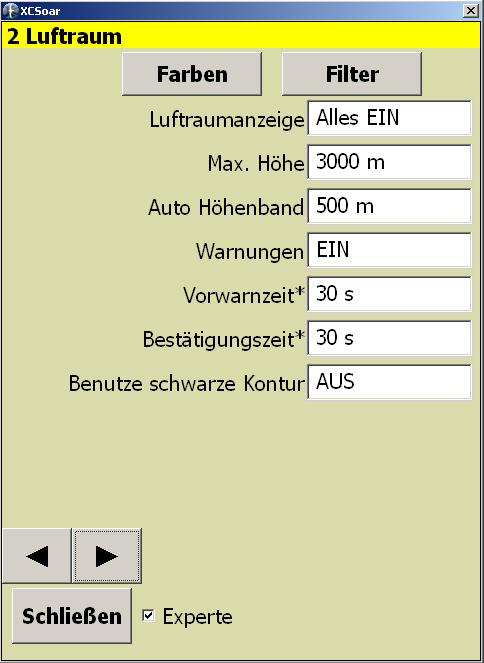
\includegraphics[width=4.5cm]{Bilder/Konfig2Luftraum.png}
\end{wrapfigure}
\begin{enumerate}
\item[Luftraumanzeige]
\item[Max.\ Höhe]
\item[Auto Höhenband]
\item[Warnungen]
\item[Vorwarnzeit$\ast$]
\item[Bestätigungszeit$\ast$]
\item[Benutze schwarze Kontur]
\end{enumerate}
\button{Farben} \qquad \button{Filter}

\subsection{Konfigurationsmenü 3 -Kartenanzeige}\label{Konfig3}
\begin{wrapfigure}{r}{5.2cm}
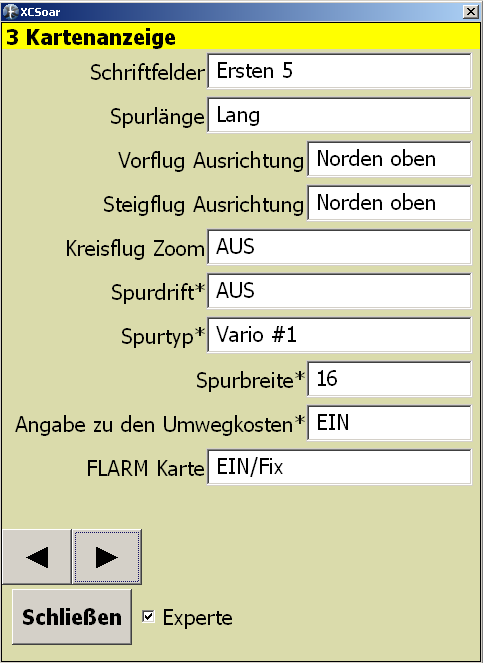
\includegraphics[width=4.5cm]{Bilder/Konfig3Kartenanzeige.png}
\end{wrapfigure}
\begin{enumerate}
\item[Schriftfelder]
\item[Spurlänge]
\item[Vorflug Ausrichtung]
\item[Steigflug Ausrichtung]
\item[Kreisflug Zoom]
\item[Spurdrift$\ast$]
\item[Spurtyp$\ast$]
\item[Spurbreite$\ast$]
\item[Angabe zu den Umwegkosten$\ast$]
\item[FLARM Karte]

\end{enumerate}

\subsection{Konfigurationsmenü 4 - Kartensymbole}\label{Konfig4}
\begin{wrapfigure}{r}{5.2cm}
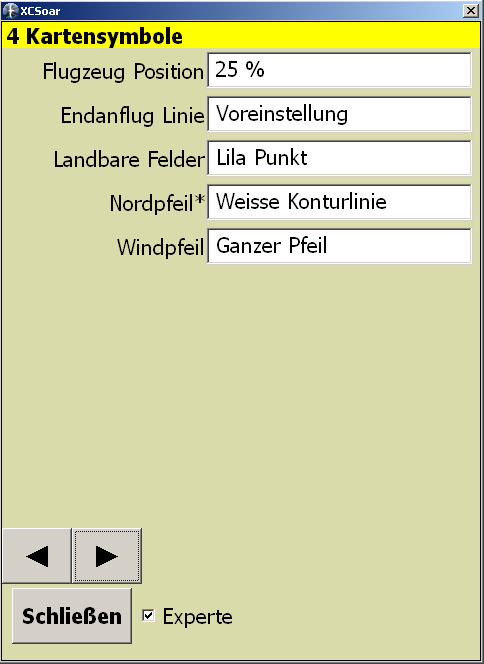
\includegraphics[width=4.5cm]{Bilder/Konfig4Kartensymbole.png}
\end{wrapfigure}
\begin{enumerate}
\item[Flugzeug Position]
\item[Endanflug Linie]
\item[Landbare Felder]
\item[Nordpfeil$\ast$]
\item[Windpfeil]
\end{enumerate}

\subsection{Konfigurationsmenü 5 - Gelände Anzeige}\label{Konfig5}
\begin{wrapfigure}{r}{5.2cm}
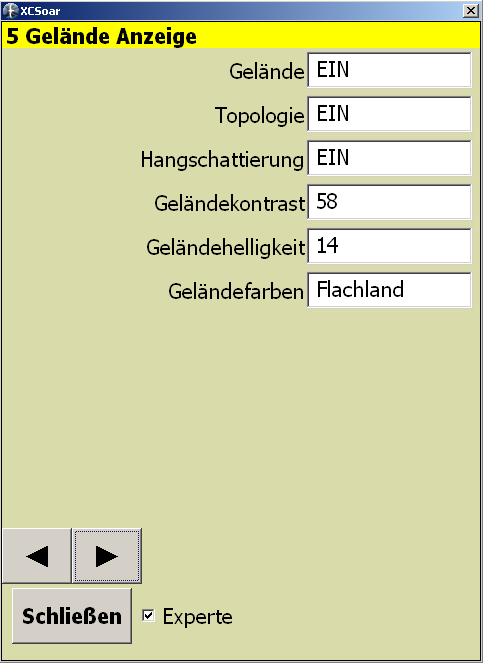
\includegraphics[width=4.5cm]{Bilder/Konfig5Gelaendeanzeige.png}
\end{wrapfigure}
\begin{enumerate}
\item[Gelände]
\item[Topologie]
\item[Hangschattierung]
\item[Geländekontrast]
\item[Geländehelligkeit]
\item[Geländefarben]
\end{enumerate}

\subsection{Konfigurationsmenü 6 - Endanflugrechner}\label{Konfig6}
\begin{wrapfigure}{r}{5.2cm}
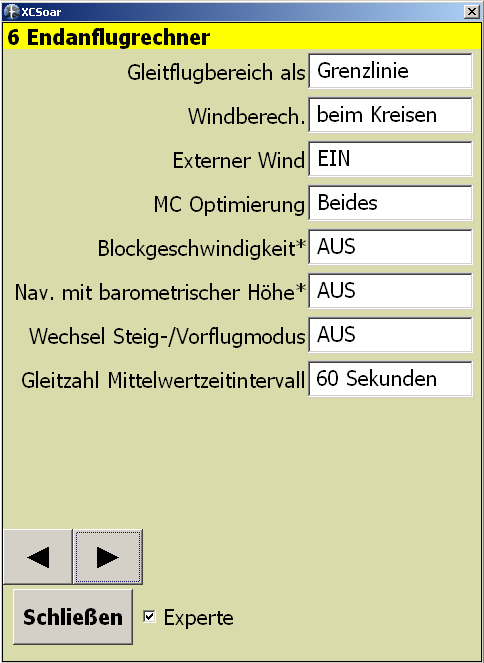
\includegraphics[width=4.5cm]{Bilder/Konfig6Endanflugrechner.png}
\end{wrapfigure}
\begin{enumerate}
\item[Gleitflugbereich als] Einstellung, wie der aktuelle Gleitbereich dargestellt werden soll: \textsf{Off} Keine Darstellung des Gleitbereiches. \textsf{Grenzlinie} Eine Linie wird um das Flugzeug gezeichnete welches den Gleitbereich darstellt. \textsf{Schattiert}: Außerhalb des Gleitbereiches wird der Bildschirm schattiert dargestellt.
\item[Windberech.]Einstellungen zur Berechnung des Windes: \textsf{ Manuell}: Der Pilot ist verantwortlich für die Eingabe des Windes. Keine automatische Berechnung \textsf{ beim Kreisen}Wind wird beim Kreisen durch Windversatz anhand GPS-Quelle ermittelt. \textsf{ZickZack}Wind kann  mithilfe eines intelligenten Variometers  errechnet werden, welches die IAS auszugeben in der Lage ist \textsf{Beides} Es werden beide vorher genannten Möglichkeiten zur Berechnung herangezogen.
\item[Externer Wind] Ein/Aus. Wenn eingeschaltet, wird der Wind von externen Geräten zur Berechnung heran- und der von \xc vorgezogen.
\item[MC Optimierung]\textsf{Endandflug} \textsf{Erwartetes mittleres Steigen} \textsf{Beides}
\item[Blockgeschwindigkeit$\ast$] Wenn aktiviert, wird im
Vorflug diejenige \textsf{MC} - Geschwindigkeit vorgeschlagen,  die für den Flug \textsl{ohne} vertikale Luftbewegung gilt. Andernfalls wird die \textsf{Delphin-Stil} Vorfluggeschwindigkeit vorgeschlagen.

    D.h.\ die \textsf{MC}-Geschwindigkeit, welche unter Berücksichtigung der vertikalen Luftmassenbewegung gilt.
\item[Nav.\ mit barometrischer Höhe$\ast$] Wenn aktiviert und vorhanden, wird die barometrische Höhe aus einem externen Gerät für alle Navigationsfunktionen verwendet.  Andernfalls wird die \textsf{GPS}-Höhe verwendet.
\item[Wechsel Steig/Vorflugmodus] \textsf{Aus} Wenn aus, dann manuell oder wie ???  \textsf{Wölbklappe} Wenn VEGA Vario und Wölbklappe gewählt ist, wird mit der Wölbklappe zwischen Kreis- und Vorflug umgeschaltet  \textsf{ man.\ Schalter} Schalter an Wölbklappe oder externer Schalter schaltet um\stop
\item[Gleitzahl Mittelwert-Zeitintervall]Zeit zur Berechnung des Mittelwertes der Gleitzahl.\footnote{Ausführliche  Beschreibung folgt später.} Standard 90sec.\
\end{enumerate}

\subsection{Konfigurationsmenü 7 - Sicherheitsfaktoren}\label{Konfig7}
\begin{wrapfigure}{r}{5.2cm}
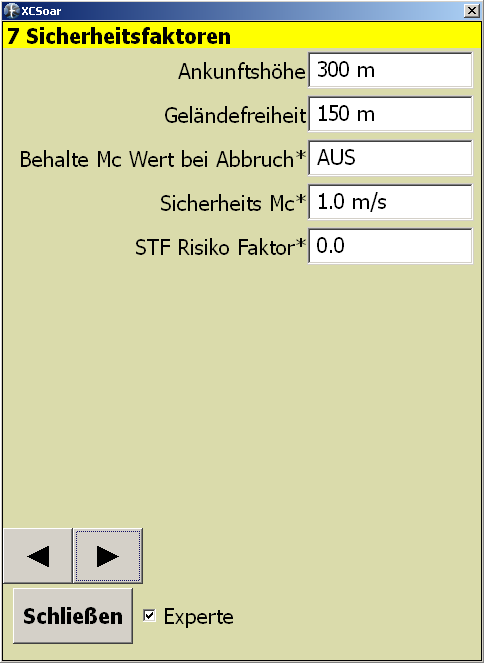
\includegraphics[width=4.5cm]{Bilder/Konfig7Sicherheistfaktoren.png}
\end{wrapfigure}
\begin{enumerate}
\item[Ankunftshöhe]
\item[Geländefreiheit]
\item[Behalte \textsf{MC} Wert bei Abbruch$\ast$]
\item[Sicherheits \textsf{MC}$\ast$]
\item[STF Sicherheitsfaktor$\ast$]
\end{enumerate}


\subsection{Konfigurationsmenü 8 - Polare}\label{Konfig8}
\begin{wrapfigure}{r}{5.2cm}
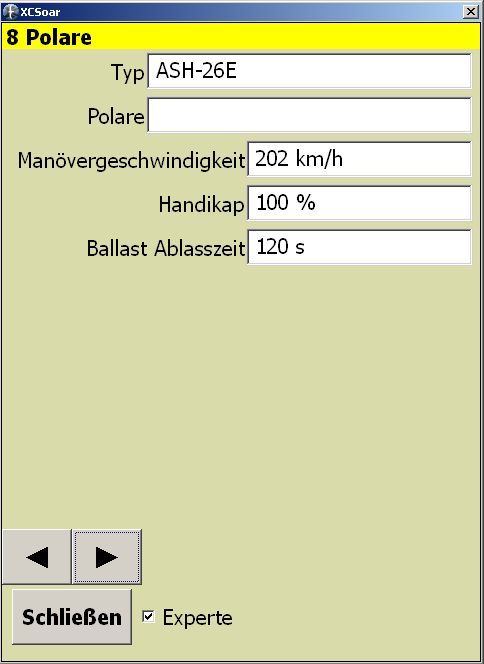
\includegraphics[width=4.5cm]{Bilder/Konfig8Polare.png}
\end{wrapfigure}
\begin{enumerate}
\item[Typ] Auswahl aus einer internen Liste möglich
\item[Polare] Wenn hier eine externe Polare gewählt werden soll, dann muß in diesem Feld die Datei mit der Polaren im \textsf{WinPilot}-Format angegeben werden.
\item[Mannövergeschwindigkeit] Auswahl der zulässigen Mannövergeschwindigkeit des gewählten Flugzeuges
\item[Handikap] Handicap - Faktor für die \textsf{OLC}-Wettbewerb Wertung
\item[Ballast Ablaßzeit] Benötigte Zeit zum kompletten Ablassen des Wasserballastes
\end{enumerate}


\subsection{Konfigurationsmenü 9 - NMEA-Anschluß (GPS-Quelle)}\label{Konfig9}
\begin{wrapfigure}{r}{5.2cm}
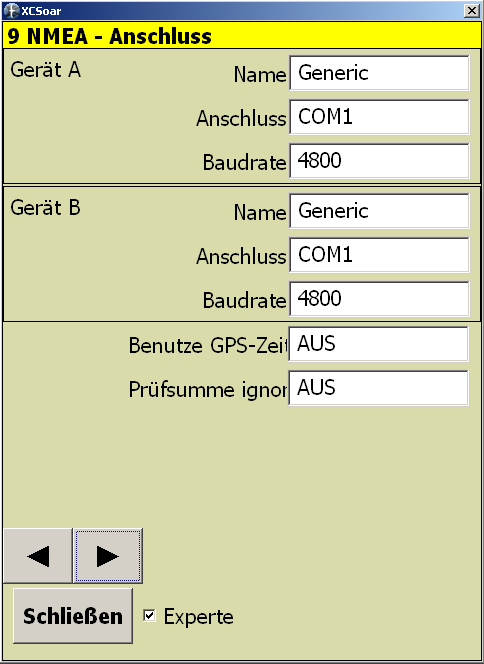
\includegraphics[width=4.5cm]{Bilder/Konfig9NMEAAnschluss.png}
\end{wrapfigure}
\begin{enumerate}
\item[Gerät A]
\begin{itemize}
\item[Name] Typ der primär angeschlossenen \textsf{GPS}-Quelle. Es sollte die zuverlässigste Quelle an Bord sein.
\item[Anschluß] Auswahl des COM-Ports. Benutzer des \textsf{Altair} müssen diesen Anschluß auf COM 3 stellen!
\item[Baudrate]\textsf{Altair} und \textsf{Vega} Benutzer sollten diese Einstellung auf 38400 stellen.
\end{itemize}
\item[Gerät B]
\begin{itemize}
\item[Name] Typ des zusätzlichen Gerätes. Es kann ein Ersatz-GPS, oder auch für andere Daten z.B.\ ein intelligentes Variometer sein.
    "Generisch" ist de Einstellung für eine \textsf{GPS}-Quelle, FLARM eingeschlossen.
\item[Anschluß]Auswahl des COM-Ports.  Benutzer des \textsf{Altair} müssen diesen Anschluß auf COM 1 stellen!
\item[Baudrate]\textsf{Altair} und \textsf{Vega} Benutzer sollten diese Einstellung auf 38400 stellen.
\end{itemize}
\item[Benutze \textsf{GPS}-Zeit]
\item[Prüfsumme ignorieren$\ast$]
\end{enumerate}



\subsection{Konfigurationsmenü 10 - Maßeinheiten}\label{Konfig10}
\begin{wrapfigure}{r}{5.2cm}
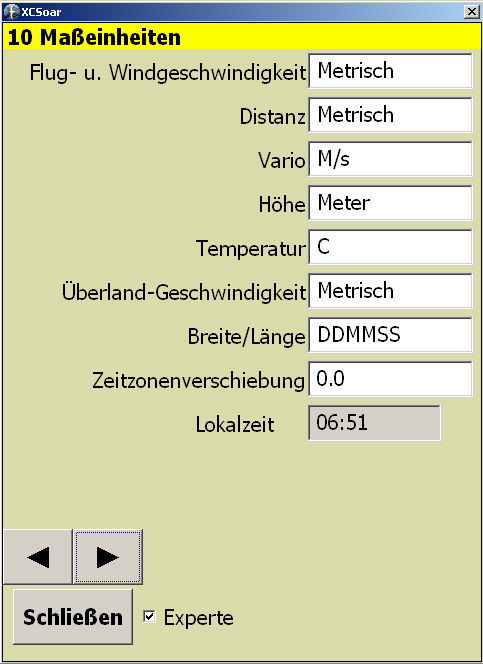
\includegraphics[width=4.5cm]{Bilder/Konfig10Masseinheiten.png}
\end{wrapfigure}
\begin{enumerate}
\item[Flug- u.\ Windgeschwindigkeit]
\item[Distanz]
\item[Vario]
\item[Höhe]
\item[Temperatur]
\item[Überland-Geschwindigkeit]
\item[Breite/Länge]
\item[Zeitzonenverschiebung]
\item[Lokalzeit]
\end{enumerate}

\subsection{Konfigurationsmenü 11 - Benutzeroberfläche}\label{Konfig11}
\begin{wrapfigure}{r}{5.2cm}
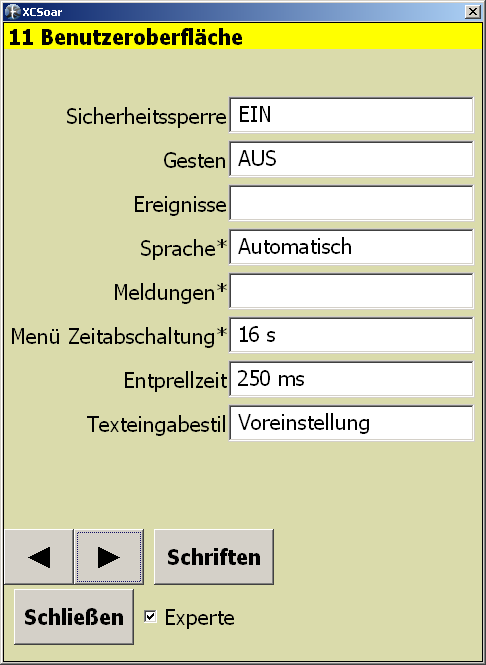
\includegraphics[width=4.5cm]{Bilder/Konfig11BenutzerOF.png}
\end{wrapfigure}
Hier erfolgt die Einstellung der Benutzer Oberfläche sowie die Auswahl der Schriften für diverse Menüs, labels etc.\
\begin{center}
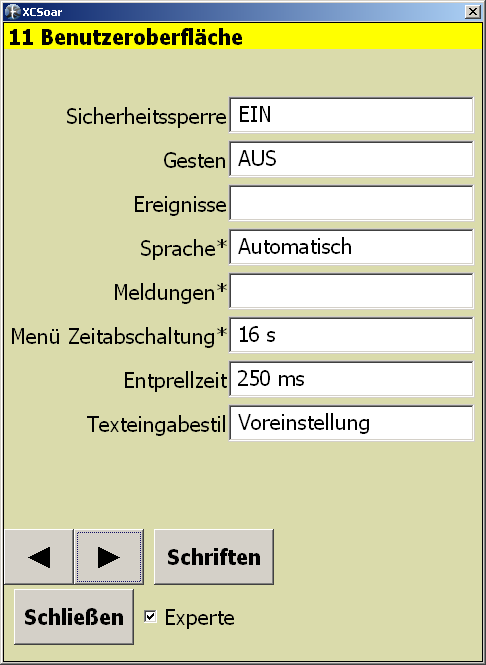
\includegraphics[width=11cm]{Bilder/Konfig11BenutzerOF.png}
\end{center}
\begin{enumerate}
\item[Sicherheitssperre:]  Ein/AUS
Einstellung, ob das Konfigurationsmenü während des Fluges  erreichbar sein soll. (Stört und macht unaufmerksam.)
\item[Gesten:] Ein/Aus
Einstellung, ob \xc auch mit Gesten auf dem Touchscreen gesteuert werden können soll
\item[Ereignisse:] Eine mögliche Eingabe-Ereignisdatei bestimmt das Menüsystem und wie \xc auf einem Knopfdruck oder z.B.\ auf ein Ereignis eines anderen externen Gerätes reagieren soll.
\item[Sprache$\ast$:] Hier wird die gewünschte Menüsprache gewählt. Es ist keine externe Sprachdatei mehr notwendig und möglich.
\item[Meldungen$\ast$:] Hier kann eine Datei angegeben werden, in festgelegt wird, welche Klänge wann und wie lange bei bestimmten Ereignissen abgespielt werden sollen.
\item[Menü Zeitabschaltung$\ast$:] Legt fest, wie lange ein Menü angezeigt wird, wenn der Benutzer keine Eingabe macht.
\item[Entprellzeit:]Minimale Zeit, nach der das System einen erneuten Tastendruck als Eingabe akzeptiert. Hilft, falls Tasten klemmen oder prellen.
\item[Texteingabestil:] Voreinstellung/Tastatur/Ranglisten Stil.
Vorgabe: Tastatur.\\
Tastatur: Inkrementelle Suche - Schnell und unkompliziert.

Ranglisten Stil: Eingabe mittels Cursorpfeilen (rechts-links, hoch-runter) entsprechende Buchstabe gefunden ist.
\end{enumerate}



\subsection{Konfigurationsmenü 12 - Anordnung}\label{Konfig12}
\begin{wrapfigure}{r}{5.2cm}
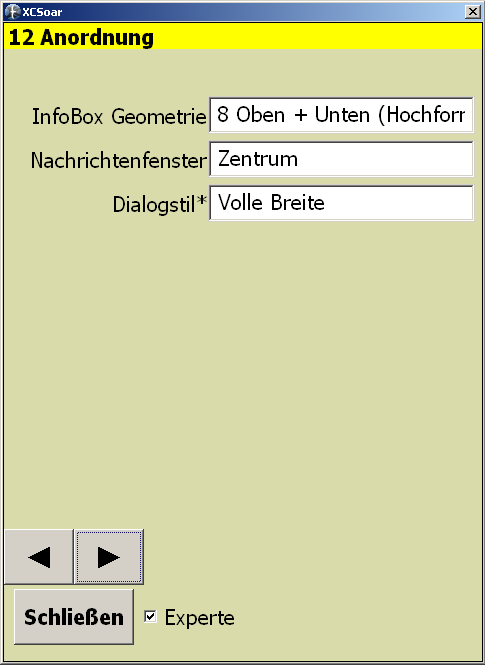
\includegraphics[width=4.5cm]{Bilder/Konfig12Anordnung.png}
\end{wrapfigure}

\begin{enumerate}
\item[Infobox Geometrie]
\item[Nachrichten Fenster $\ast$]
\item[Dialogstil $\ast$]
\end{enumerate}

\subsection{Konfigurationsmenü 13 - Flarm und andere Anzeigen}\label{Konfig13}
\begin{wrapfigure}{r}{5.2cm}
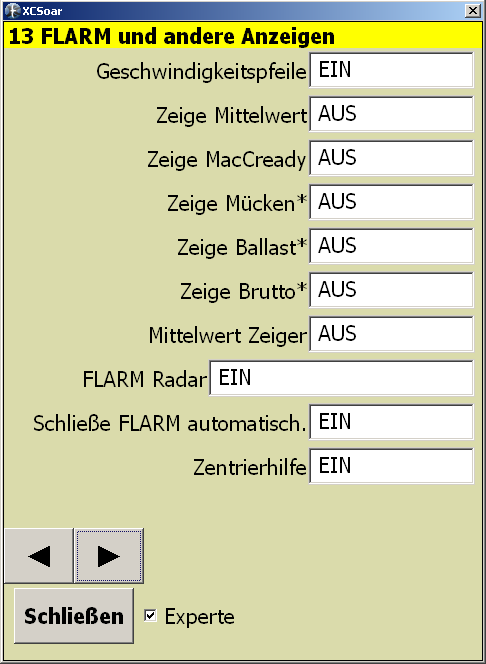
\includegraphics[width=4.5cm]{Bilder/Konfig13FLARM.png}
\end{wrapfigure}
\begin{enumerate}
\item[Geschwindigkeitspfeile]
\item[Zeige Mittelwert]
\item[Zeige Mc Cready-Wert]
\item[Zeige Mücken]
\item[Zeige Ballast]
\item[Zeige Brutto]
\item[Mittelwert Zeiger]
\item[Flarm Radar]
\item[Schließe FLARM automatisch]
\item[Zentrierhilfe]
\end{enumerate}

\subsection{Konfigurationsmenü 14 - Standard Wettbewerbsregeln}\label{Konfig14}
\begin{wrapfigure}{r}{5.2cm}
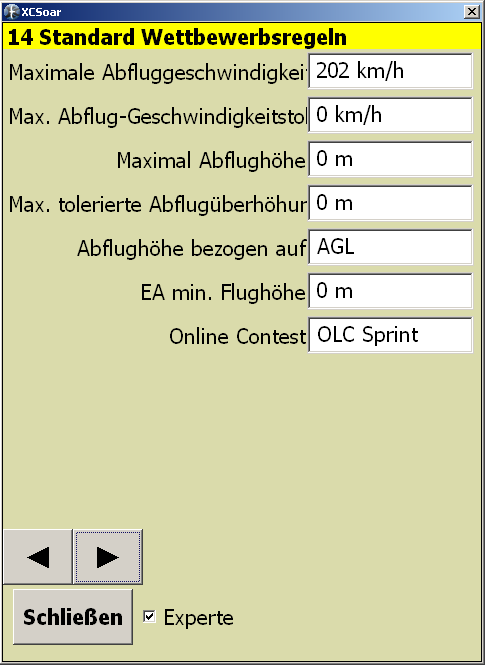
\includegraphics[width=4.5cm]{Bilder/Konfig14Wettbewerb.png}
\end{wrapfigure}
\begin{enumerate}
\item[Maximale Abfluggeschwindigkeit]
\item[Max.\ Abflug-Geschwindigkeitstoleranz]
\item[Maximale Abflughöhe]
\item[Max.\  tolerierte Abflughöhung ]
\item[Abflughöhe bezogen auf]
\item[EA min.\ Flughöhe]
\item[Online Contest]
\end{enumerate}

\subsection{Konfigurationsmenü 15 - Infoboxen}\label{Konfig15}
\begin{wrapfigure}{r}{5.2cm}
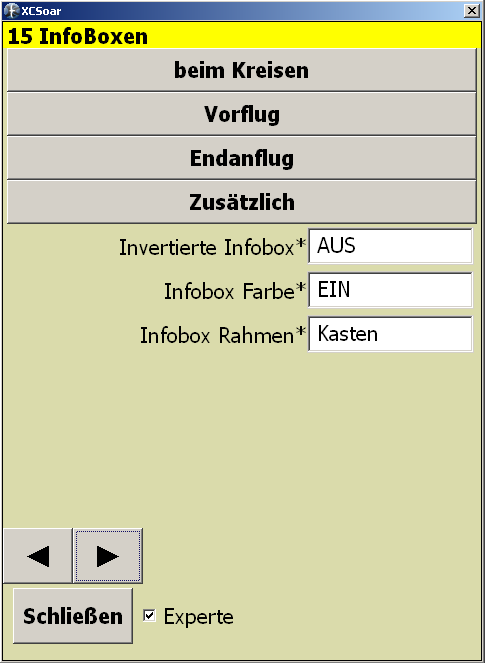
\includegraphics[width=4.5cm]{Bilder/Konfig15Infoboxen.png}
\end{wrapfigure}
\begin{enumerate}
\item[beim Kreisen]
\item[Vorflug]
\item[Invertierte Infobox$\ast$]
\item[Infobox Farbe$\ast$]
\item[Zusätzlich$\ast$]
\end{enumerate}

\subsection{Konfigurationsmenü 16 - Logger}\label{Konfig16}
\begin{wrapfigure}{r}{5.2cm}
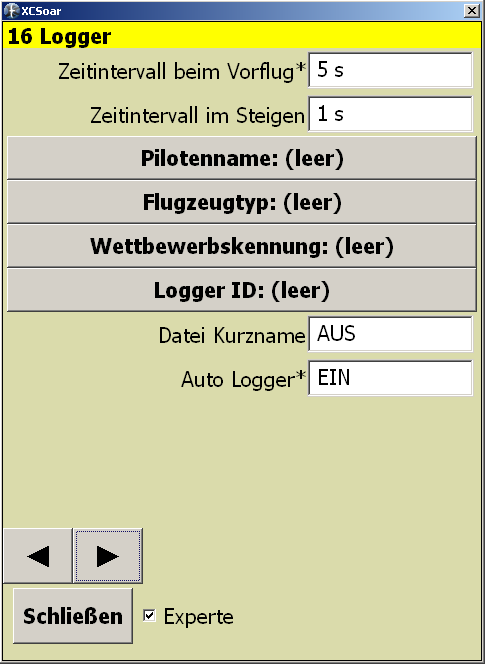
\includegraphics[width=4.5cm]{Bilder/Konfig16Logger.png}
\end{wrapfigure}
\begin{enumerate}
\item[Zeitintervall beim Vorflug$\ast$]
\item[Zeitintervall beim Steigen]
\item[Pilotenname]
\item[Flugzeugtyp]
\item[Wettbewerbskennung]
\item[Logger ID]
\item[Datei Kurzname] Der Loggerschrieb des Fluges wird in eine Datei geschrieben
Diese Einstellung legt fest, ob kurze oder lange IGC-Dateinamen verwendet werden:
Kurz: 81HXABC1.IGC,  Lang: 2008-01-18-XXX-ABC-01.IGC
\item[Auto Logger$\ast$] Aktiviert den automatischen Loggerschrieb beim Abheben und Landen. Achtung: Bei Gleitschirmen muß dies Feld auf Aus stehen, da die Geschwindigkeiten i.d.R.\ zu gering sind.
\end{enumerate}

\subsection{Konfigurationsmenü 17 - Experimental}\label{Konfig17}
\begin{wrapfigure}{r}{5.2cm}
\includegraphics[width=4.5cm]{Bilder/Konfig17Experimental.png}
\end{wrapfigure}
\begin{enumerate}
\item[Bisher ohne Funktion]
\end{enumerate}

%\input{DataFiles.tex}                                     % Im Bau Sehr wichtig 
%\newpage
%\input{Entwicklung-und-Entstehung.tex}       % Im Bau  - unwichtig 
%\begin{small}
 %\input{GnuGeneralPublicLicense.tex}          % Fertig
%\end{small}
\tableofcontents
\printindex
\end{document}
